
\subsection{Usage Overview}

\begin{figure*}
	\centering
	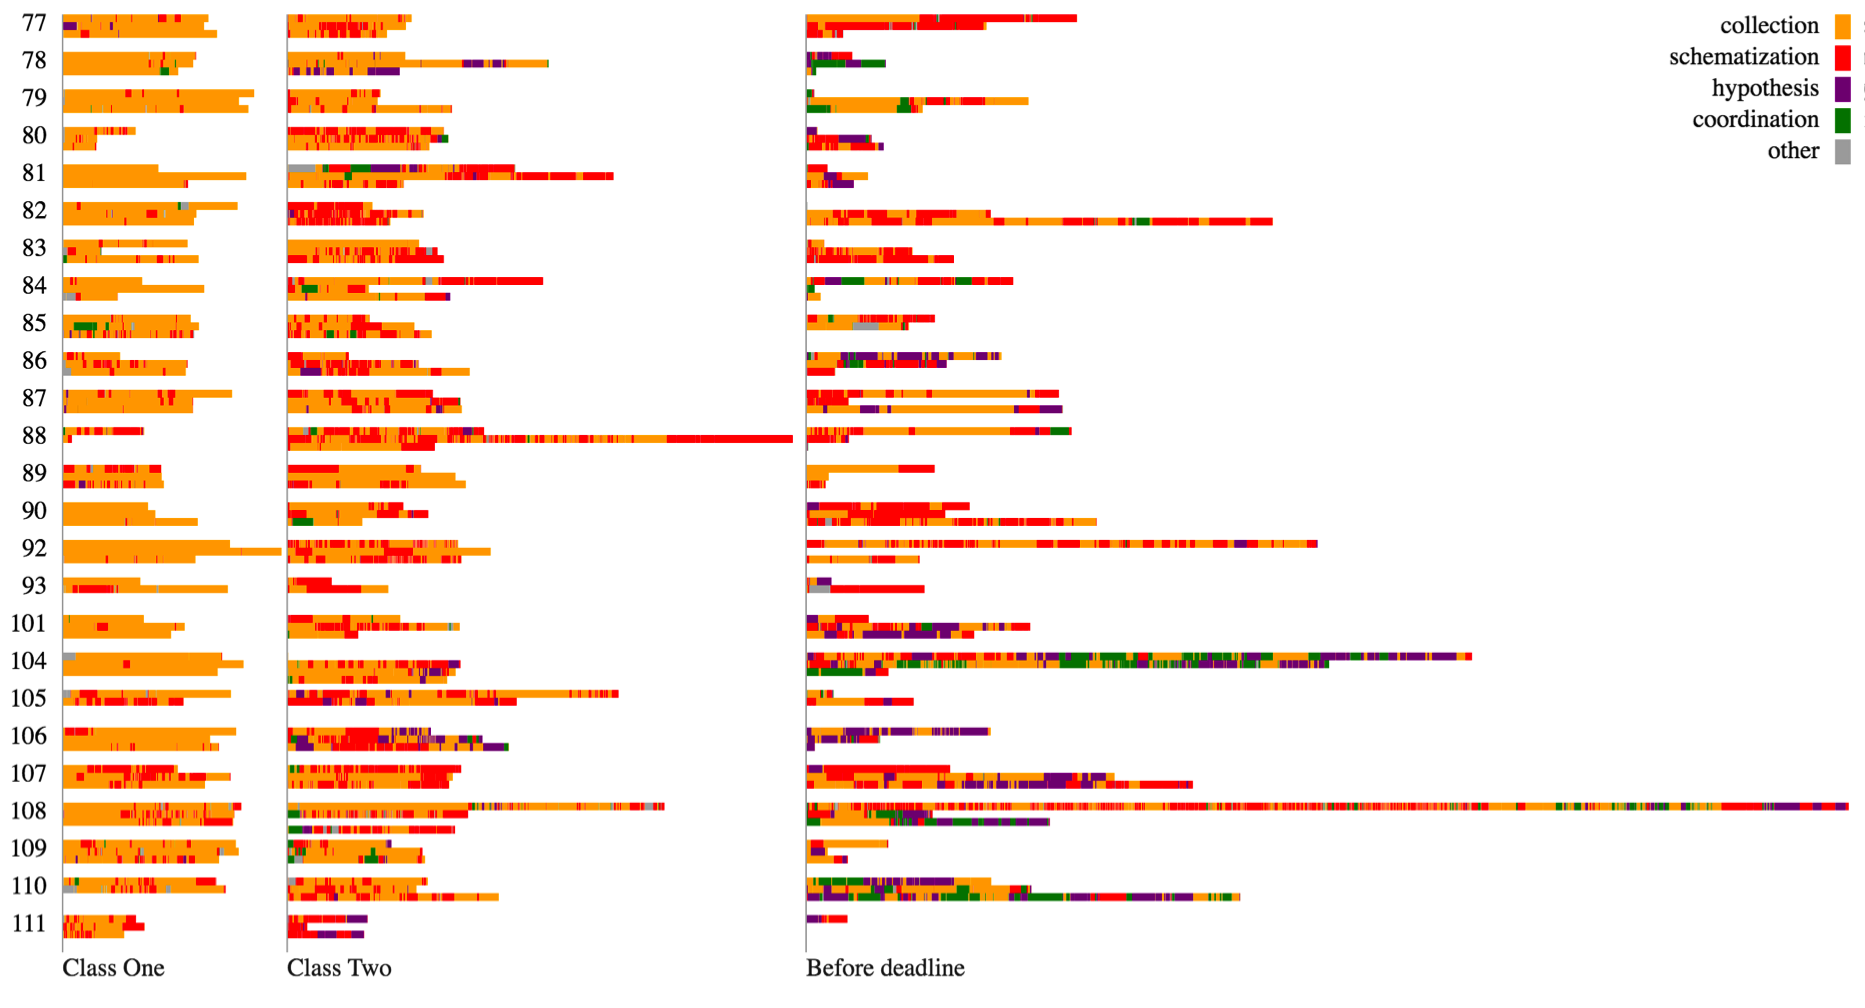
\includegraphics[height=2.5in]{img/phase_sequence}
	\caption{Teams' activity patterns of evidence collection, evidence schematization, hypothesis generation, and overall coordination.}
\end{figure*}



From the system log we made an approximation of the time teams spent on each phase (Figure~\ref{fig:phase_time}). Note that there could be multiple error sources. For example, we actually only capture discrete log events on a tool, and we approximate the duration time assuming that the user keeps on working on that tool until the next log event occurs on another tool (but we discard the time if the interval between two log events is bigger than a threshold). Also we assume that people working with annotation are in evidence collection, and people working with visualizations are in evidence schematization, but in fact no clear boundary exist between the phases. For instance, participants might be schematizing and analyzing evidence as well when they are reading documents and making annotations. 

Yet still, there are several things we can learn from such approximation. For instance, nearly all teams spent most time on tools for evidence collection, less on tools for evidence schematization, and least on tools for hypothesis generation. This seems in contradict with theory; people should spend more time on high level sensemaking activities and focus on the problem itself rather than the underlying data. While evidence collection itself is time-consuming as it requires large amounts of manual input, more advanced input facilities is needed to reduce the time in this phase. 

We use time spent on the history tool and message tool as proxy of overall coordination, although it is only a small portion in real team coordination, because teams can talk directly face-to-face in our study. 

From the system log, we can clearly see that user activities are most intense in three time periods: during class one, during class two, and before project deadline. In class time, students are obviously working together; but when outside class, teams have different choices. 


\begin{figure}
	\centering
	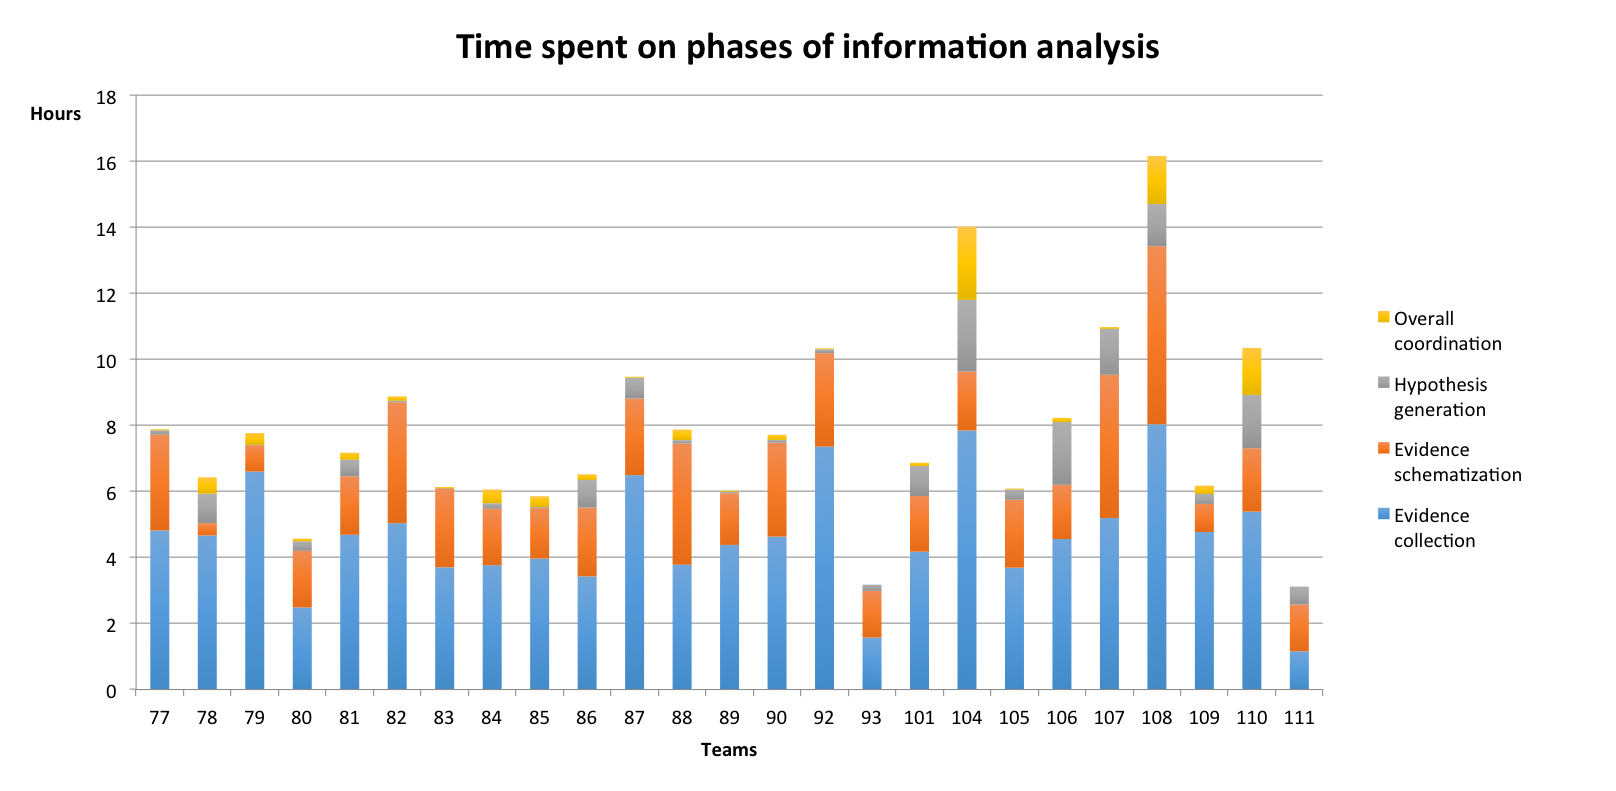
\includegraphics[height=1.5in]{img/phase_time}
	\caption{Time spent on each phase of information analysis.}
\end{figure}

We then look in more detail into the sequence of user activities, in an attempt to find if there exists any behavior patterns between teams, as shown in Figure~\ref{fig:phase_sequence}. Since there are obviously three active usage periods, we align activities into three phases: in the first class, in the second class, and before project deadline. Note that this graph only shows the order of activities performed by participants and spare time between activities (if any) is removed to reduce graph sparsity. We find that teams tend to have a behavior swift between phases. In the first phase, teams spent most time in evidence collection. In Phase Two, teams started to engage in evidence schematization. And teams apparently worked more in hypothesis generation activities. For teams working remotely, they also utilized coordination tools. 

Unlike the sensemaking model \cite{?}, which implies a linear process in information analysis (analysts first specify problems and requirements, then collect information, followed by schematization and analysis, and finally produced a report), we find that teams have a more flexible workflow. They do not wait until all information is collected to do analysis, nor do they hold generating hypotheses until analysis is done. Especially starting from Phase Two (and some teams started even earlier e.g. Team 107) when teams felt they had collected ``good enough'' evidence, they started to use the visualization tools and hypothesis tools. And they switch back and forth from one activity to the other frequently. Especially in later stage, teams seemed to work on the three activities in parallel.  

\hl{TODO: describe the pattern in more details}

In students' reflection, they believe that the integrated analytic environment that CAnalytics provides makes their work more effective and efficient. 

\begin{quote}
	When we didn’t have CAnalytics, we had a lot of different word documents that we had to share with each other in google documents. (P155)
\end{quote}

\begin{quote}
	our team is doing better because CAnalytics as a whole lets us see, analyze, and make conclusions all within one location. (P123)
\end{quote}







\begin{quote}
	\textit{`CAnalytics seemed like the beta-version of an analyst's notebook that multiple people could work on at once...It was like having an analyst's version of a Google Doc.'} (P21)
\end{quote}






\begin{quote}
\textit{`It was much easier to coordinate as a team with CAnalytics because we could all work on the same system at the same time'}
\end{quote}

% integrated environment
Students thought CAnalytics was a better integrated analytic environment. It provided the analytic tools the team needed and kept all analytic products in one shared place. With traditional tools, however, students recalled that they had to map out different types of data objects in specialized tools, e.g. mapping in Google Maps, timeline and network in Analyst's Notebook, table and document in Google Doc. The scattering of resources available added difficulty of coordination.



